
\epigraph{\emph{\noindent
This remark is based on a ``theorem'', which as far as I know has never been proven, but which I cannot imagine could be wrong.
}}
{
    --- Steven Weinberg, 1979~\autocite{weinbergPhenomenologicalLagrangians1979a}
}


\section{Pion stars}

Stars and planets have long been one of the main driving engines behind the developments of physics.
A lot of early mathematics was developed to navigate using the stars and to predict the seasons and the phases of the moon.
One of the most important confirmations of Newton's laws of motion and gravity was their prediction of Kepler's laws from more basic assumptions.
Kepler's laws concern the orbits of planets around the sun.
They are empirical observations made by Kepler after studying the data gathered by Tycho Brahe.
Likewise, the successor to Newton's law of gravitation, Einstein's general relativity, was first shown to be more accurate than its predecessor by predicting the drift of the perihelion of the orbit of Mercury~\autocite{carrollSpacetimeGeometryIntroduction2019}.
The radiation of the Sun has been part of the development of the theory of light and thermal radiation~\autocite{hemmerTermiskFysikk2002}.
To understand the process that fuels the Sun, we had to develop special relativity, in which mass is described as just another form of energy, as well as quantum mechanics and the theory of nuclear fusion.
Observations of the neutrinos resulting from these processes lead to the discovery of neutrino oscillations~\autocite{prialnikIntroductionTheoryStellar2000}.
Today, this is one of the few empirical observations in physics that conflict with the standard model of particle physics.
The Sun might therefore still be part of the development of new fundamental physics.

Even after a star has depleted its fusion fuel it can remain an object of great interest.
Stars with less mass than around $10$ times that of the sun, $M_\odot$, will towards the end of their active life shed most of their outer layers, leaving behind an inert white-hot mass only supported by the pressure of its electrons.
These are called \emph{white dwarfs}.
One cubic centimeter of the material that makes up white dwarfs weighs more than a ton.
Sirius B, the fainter companion to Sirius, is a white dwarf.
A characteristic property of fermions, such as electrons, is the Pauli exclusion principle, which states that two identical fermions may not occupy the same quantum state.
This leads to \emph{degeneracy pressure}, where tightly packed fermions exert pressure, not as a result of any interaction, but solely due to this exclusion principle.
It is due to this effect that electrons can withstand the gravitational pull of white dwarfs.
Type Ia supernovae happen as white dwarfs reach their upper mass limit, the Chandrasekhar limit, and are invaluable in mapping the distances of our universe~\autocite{carrollSpacetimeGeometryIntroduction2019}.
White dwarfs, together with the even more dense \emph{neutron stars}, are collectively known as \emph{compact stars}.
Neutron stars are left after the supernova explosions of massive stars~\autocite{prialnikIntroductionTheoryStellar2000}.
They were first predicted solely on theoretical backgrounds and later discovered in the form of pulsars, rotating neutron stars with frequencies below a tenth of a second, where strong magnetic fields act as particle accelerators~\autocite{prialnikIntroductionTheoryStellar2000}.
Compact stars are some of the most extreme environments in our universe, and as such, they are excellent places for exotic physics to happen.

Recently, a new class of compact stars has been proposed, called pion stars~\autocite{andersenBoseEinsteinCondensationPion2018,brandtNewClassCompact2018,carignanoScrutinizingPionCondensed2017}.
These stars are composed of a pion condensate.
As pions are bosons, they do not obey the Pauli exclusion principle, and pion stars cannot rely on degeneracy pressure to support themselves.
Instead, the pions must have a repulsive interaction to exert such pressure.
Pion stars are, as yet, only a theoretical proposal.
However, if history is to be of any guidance, that does not mean there aren't valuable insights to be gained from researching them.
Only with a model of how pion stars behave can we ever hope to detect them.
To that end, we need a theory of the matter that makes up such a star.




\section{The standard model, QCD, and effective theories}


The Standard Model of particle physics is the totality of what particle physicists are confident they understand concerning the fundamental building blocks of our universe.
It is arguably the most successful scientific theory of all time and makes fantastically accurate predictions of the behavior of fundamental particles.
In combination with general relativity, it is our best framework for explaining how the world works.
The Standard Model is a quantum field theory (QFT) and describes both the elementary matter particles and the forces between them as excitations in quantum fields permeateing all space-time.
These fields and their dynamics are captured in the \emph{Lagrangian density}, or just Lagrangian, of the model.
In deceivingly compact notation, this can be written
%
\begin{equation}
    \label{standard model lagrangian}
    \Ell_\text{SM}
    =
    \bar \psi_i \slashed{ D }_{ij}  \psi_j
    - \frac{1}{4} F_\alpha^{\mu\nu} F^\alpha_{\mu \nu}
    - \left( 
        \bar \psi_{L, i} \Phi Y_{ij} \psi_{R, j}
        + \hc
    \right)
    + |D_{\mu} \Phi |^2 + \Ve(\Phi).
\end{equation}
%
Here, the $\psi_i$'s are the fermionic fields, of which atoms are made.
The forces are encoded in $D$ and $F$, and their form are determined by the \emph{gauge group} of the Standard Model, $ \Lie{SU}{3}_c\times \Lie{SU}{2}_L\times \Lie{U}{1}_Y$.
This is the set of all gauge symmetries.
More generally, symmetries such as gauge symmetries or the Lorentz symmetry of special relativity greatly constrain the form of $\Ell_\text{SM}$.
Lastly, $\Phi$ is the Higgs-field, which interaction with other fields are responsible for the mass of particles~\autocite{carrollWorldEverydayExperience2013,schwartzQuantumFieldTheory2013}.
The fundamental particles of the Standard Model are excitations in the fields of \autoref{standard model lagrangian} and are illustrated in \autoref{fig: standard model}~\autocite{griffithsIntroductionElementaryParticles2008,schwartzQuantumFieldTheory2013}
If we include the masses of neutrinos in the Standard Model, it has 26 free parameters~\autocite{kramerStandardModelParticle2017}.
We should, in principle, be able to derive all of particle physics from the Standard Model together with these parameters, and from that subsequently chemistry and all other physical sciences.
In practice, however, we must often resort to domain-specific models, which might be guided by the Standard Model, but ultimately are independent.
However, unless you hope to supplant the Standard Model, no such model should violate it.
The Standard Model obeys general constraints such as the conservation of energy and the speed of light as the ultimate speed limit.
These constraints are powerful guiding lights as we seek to explore physics.



\begin{figure}[!htb]
    \centering
    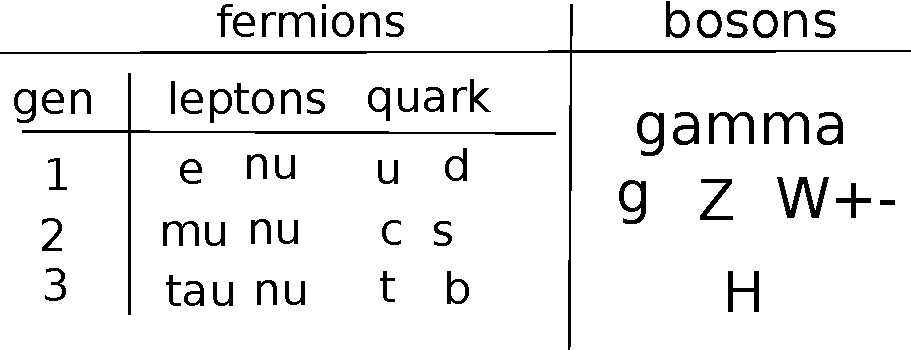
\includegraphics[width=.7\textwidth]{figurer/standard_model.pdf}
    \caption{
        The particles of the standard model come in two main groups.
        The bosons include the force-carrying gauge particles and the Higgs boson (H).
        The fermions make up matter, and come in three ``generations''.
    }
    \label{fig: standard model}
\end{figure}


The part of the Standard Model that describes the interaction of quarks via the strong force, mediated by the gluons, is called \emph{quantum chromodynamics} (QCD).
Quarks are the building blocks of the nuclear particles, protons and neutrons, and the nuclear force that binds together atoms is a result of QCD.
A complete understanding of this theory is of great interest.
However, the fact that the force mediated by gluons is so strong greatly limits our understanding.
This is because our main technique for handling quantum field theories, perturbation theory, fails.
In perturbation theory, we rely on interactions being weak.
This is quantified by an expansion parameter, $\alpha$, to which the strength of each interaction is proportional.
If $\alpha<1$, then each such interaction in a process will suppress it by a factor $\alpha$.
The scattering of two particles is then calculated as a sum of all possible processes---combinations of interactions between the fields---that could lead to that event.
Processes with more interactions will contribute less to the total sum, as each interaction suppresses it by $\alpha$.
Each process is illustrated by a Feynman diagram, in which particles come in from the left, interact via \emph{virtual particles}, then leave to the right.
The process of electron-muon scattering in quantum electrodynamics (QED) is given by
%
\begin{equation*}
\begin{tikzpicture}[baseline=(c)]
    \begin{feynman}
        \vertex (a1) at (0, 0);
        \vertex (b1) at (1, 0);
        \vertex (c1) at (2, 0);
        %
        \vertex (a2) at (0, -1);
        \vertex (b2) at (1, -1);
        \vertex (c2) at (2, -1);
        %
        \vertex[left=0.1cm of a1] {$e^-$};
        \vertex[right=0.1cm of c1] {$e^-$};        
        \vertex[left=0.1cm of a2] {$\mu^-$};
        \vertex[right=0.1cm of c2] {$\mu^-$};
        %
        \node [blob] (c) at (1, -.5);
        %
        \diagram*{
            {[edges=Fermion]
            (a1) -- (c) -- (c1),
            (a2) -- (c) -- (c2)},
        };
    \end{feynman}
\end{tikzpicture}
=
\underbrace{\, \,
 \begin{tikzpicture}[baseline=(c)]
    \begin{feynman}
        \vertex (a1) at (0, 0);
        \vertex (c1) at (2, 0);
        \vertex (a2) at (0, -1);
        \vertex (c2) at (2, -1);
        \vertex (x) at (1, -.2);
        \vertex (c) at (1, -.5);
        \vertex (y) at (1, -.8);
        \diagram*{
            {[edges=Fermion]
            (a1) -- (x) -- (c1),
            (a2) -- (y) -- (c2)},
            {[edges=photon]
            (x) -- (y)}
        };
    \end{feynman}
\end{tikzpicture}
\, \,
}_{\propto {\alpha}}
+
\underbrace{ \, \,
\begin{tikzpicture}[baseline=(c)]
    \begin{feynman}
        \vertex (a1) at (0, 0);
        \vertex (d1) at (2.4, 0);
        \vertex (a2) at (0, -1);
        \vertex (d2) at (2.4, -1);
        \vertex (x) at (.8, -.2);
        \vertex (y) at (.8, -.8);
        \vertex (x2) at (1.6, -.2);
        \vertex (y2) at (1.6, -.8);
        \vertex (c) at (.8, -.5);
        \diagram*{
            {[edges=Fermion]
            (a1) -- (x) -- (x2) -- (d1),
            (a2) -- (y) -- (y2) -- (d2)},
            {[edges=photon]
            (x) -- (y),
            (x2) -- (y2)}
        };
    \end{feynman}
\end{tikzpicture}
+
\begin{tikzpicture}[baseline=(c)]
    \begin{feynman}
        \vertex (a1) at (0, 0);
        \vertex (c1) at (2, 0);
        \vertex (a2) at (0, -1);
        \vertex (c2) at (2, -1);
        \vertex (x) at (1, 0);
        \vertex (l1) at (1, -.3);
        \vertex (c) at (1, -.5);
        \vertex (l2) at (1, -.7);
        \vertex (y) at (1, -1);
        \diagram*{
            {[edges=Fermion]
            (a1) -- (x) -- (c1),
            (a2) -- (y) -- (c2),
            (l1) --[half left, looseness=1.8] (l2) --[half left, looseness=1.8] (l1),
            },
            {[edges=photon]
            (x) -- (l1),
            (l2) -- (y)
            }
        };
    \end{feynman}
\end{tikzpicture}
+
\begin{tikzpicture}[baseline=(c)]
    \begin{feynman}
        \vertex (a1) at (0, 0);
        \vertex (b1) at (.5, -.1);
        \vertex (c1) at (1, -.2);
        \vertex (d1) at (1.5, -.1);
        \vertex (e1) at (2, 0);
        \vertex (a2) at (0, -1);
        \vertex (c2) at (1, -.8);
        \vertex (e2) at (2, -1);
        \vertex (c) at (0, -.5);
        \diagram*{
            {[edges=Fermion]
            (a1)--(c1)--(e1),
            (a2)--(c2)--(e2)},
            (b1) --[boson, quarter left] (d1),
            (c1) --[boson] (c2)
        };
    \end{feynman}
\end{tikzpicture}
\, \,
}_{\propto {\alpha}^2}
+ \dots.
\end{equation*}
%
In QED, the expansion parameter is the fine structure constant, $\alpha = e^2/(4 \pi)$ where $e$ is the elementary electrical charge.
In renormalized theories, such as QED, this parameter is dependent on the energy scale $Q$ the processes happen at.
This is called the \emph{running} of the coupling.
At $Q = 0$, $ \alpha \approx 7 \times 10^{-3}$, and only a few orders in perturbation theory will therefore give highly precise and accurate results.\footnote{
    The series expansion in terms of coupling constants is, strictly speaking, not a converging series, but rather an asymptotic series.
    We can see this by considering the consequences of exchanging $\alpha$ for $-\alpha$.
    Such a theory would be unstable as like charges would attract.
    This implies any expansion in $\alpha$ has a zero radius of converge~\autocite{dysonDivergencePerturbationTheory1952}.
    We must therefore consider the sum of Feynman-diagrams as an asymptotic series, which yields a good approximation \emph{if terminated soon enough}~\autocite{floryHowLearnedStop2012}.
}

In QCD, we have no such luck.
The equivalent of the fine-structure constant in QCD, $\alpha_s$, increases as the energy scale decreases, in contrast to $\alpha$.
As a consequence, perturbation theory breaks down for $Q$ below around $1\,\text{GeV}$.
This includes everything but the most extreme situations in the universe.
At such energy scales, quarks and gluons are bound together as \emph{hadrons}.
Hadrons are divided into two classes, \emph{baryons} and \emph{mesons}.
The nucleons making up the core of atoms---the neutron and the proton---are among the baryons.
Baryons are made up of three quarks, while mesons are made of two.
The lightest meson, the pion, was predicted theoretically by Hideki Yukawa as the carrier of the nuclear force and later discovered by Cecil Powell \emph{et al.}~\autocite{griffithsIntroductionElementaryParticles2008}.

We are unable to directly and analytically describe QCD at low energies due to this breakdown of perturbation theory.
There are numerical schemes, namely lattice QCD, which allow for calculations of low-energy QCD.
These methods rely on large amounts of computing power, and as we will detail further, have problems with important cases of interest due to the so-called sign problem.
We will tackle the problem by using an \emph{effective field theory}.
When constructing an effective field theory, we come to terms with the fact that we do not know all physics.
Instead, we settle for a description of the most important parts.
In modern physics, effective field theories have become a ubiquitous tool and are employed in both condensed matter physics and high-energy physics.
In fact, it is now believed that the Standard model itself is an effective field theory, a low energy description of a more complete theory~\autocite{pencoIntroductionEffectiveField2020,weinbergDevelopmentEffectiveField2021}.
The ``theorem'' Weinberg discusses in the opening quote of this chapter describes why effective field theories are such powerful tools.
In short, it states that quantum field theories alone contain very little information, and thus can model almost everything.
If we write down the most general Lagrangian, we have not made more than very basic assumptions~\autocite{weinbergPhenomenologicalLagrangians1979a}.
This will be our guiding philosophy when constructing \emph{chiral perturbation theory} (\chpt\,), the effective theory of mesons.




\section{Thermodynamics and the physics of compact stars}

In the same way that we are lucky nature allows us to ignore high-energy effects and instead use an effective theory of low-energy interactions, statistical mechanics and thermodynamics allow us to describe composite systems containing a large number of degrees of freedom with only a few variables.
Instead of perfectly describing all degrees of freedom and their interactions, we consider what the average system would look like.
As long as the system is large enough and is in thermal equilibrium, which means that the system is in a stable state without flows of matter or energy where the thermodynamic variables are well-defined, then this gives an astonishingly effective and economical description of the system.
There are several choices for free variables when describing a thermodynamic system.
The temperature of a system, $T$, determines whether energy would flow to or from that system to a different system with a different temperature $T'$.
In our description of pion stars, we will assume $T = 0$, as they are much denser than they are hot and thermal effects thus can be neglected to a first approximation.
We work in the \emph{grand canonical ensamble}, in which we consider the system coupled to a source of \emph{conserved charges}, such as electrical charge, or particle number in non-relativistic physics.
By adjusting the chemical potential, $\mu$, corresponding to a conserved charge, $Q$, we set how energetically favorable it is to add a new charge to the system, and thus the charge density of a typical system.

In our case, all relevant thermodynamic variables are independent of the volume of the system, and chemical potential is thus the only free variable.
Therefore, it determines all other variables, such as energy density $u$ and pressure $p$.
This relationship, which can be stated implicitly on the form $f(p, u, \mu) = 0$, is called the \emph{equation of state} of the system.
We will use the Tolman-Oppenheimer-Volkoff (TOV) equation to model pion stars.
This is based on general relativity and describes a static sphere of matter and energy in which the outward push of its internal pressure is balanced by gravity.
The TOV equation needs the equation of the state of the substance it describes as an input.
To model pion stars, then, we must calculate the equation of state of the pion condensed-phase of QCD.



\section{The QCD phase diagram}

A phase diagram illustrates the properties of a medium under different circumstances.
The pion condensed phase is only one part of the rich phase diagram of QCD, an active area of research.
Our understanding of it is far from complete due to the difficulties of working with the strong force.
\autoref{fig: phase diagram QCD} shows a rough sketch of our current understanding of the QCD phase diagram.
The axes are temperature $T$, baryon chemical potential $\mu_B$, and isospin chemical potential $\mu_I$.
The baryon and isospin chemical potentials quantify the abundance of quarks compared to antiquarks and up quarks compared to down quarks, respectively.

\begin{figure}[!htb]
    \centering
    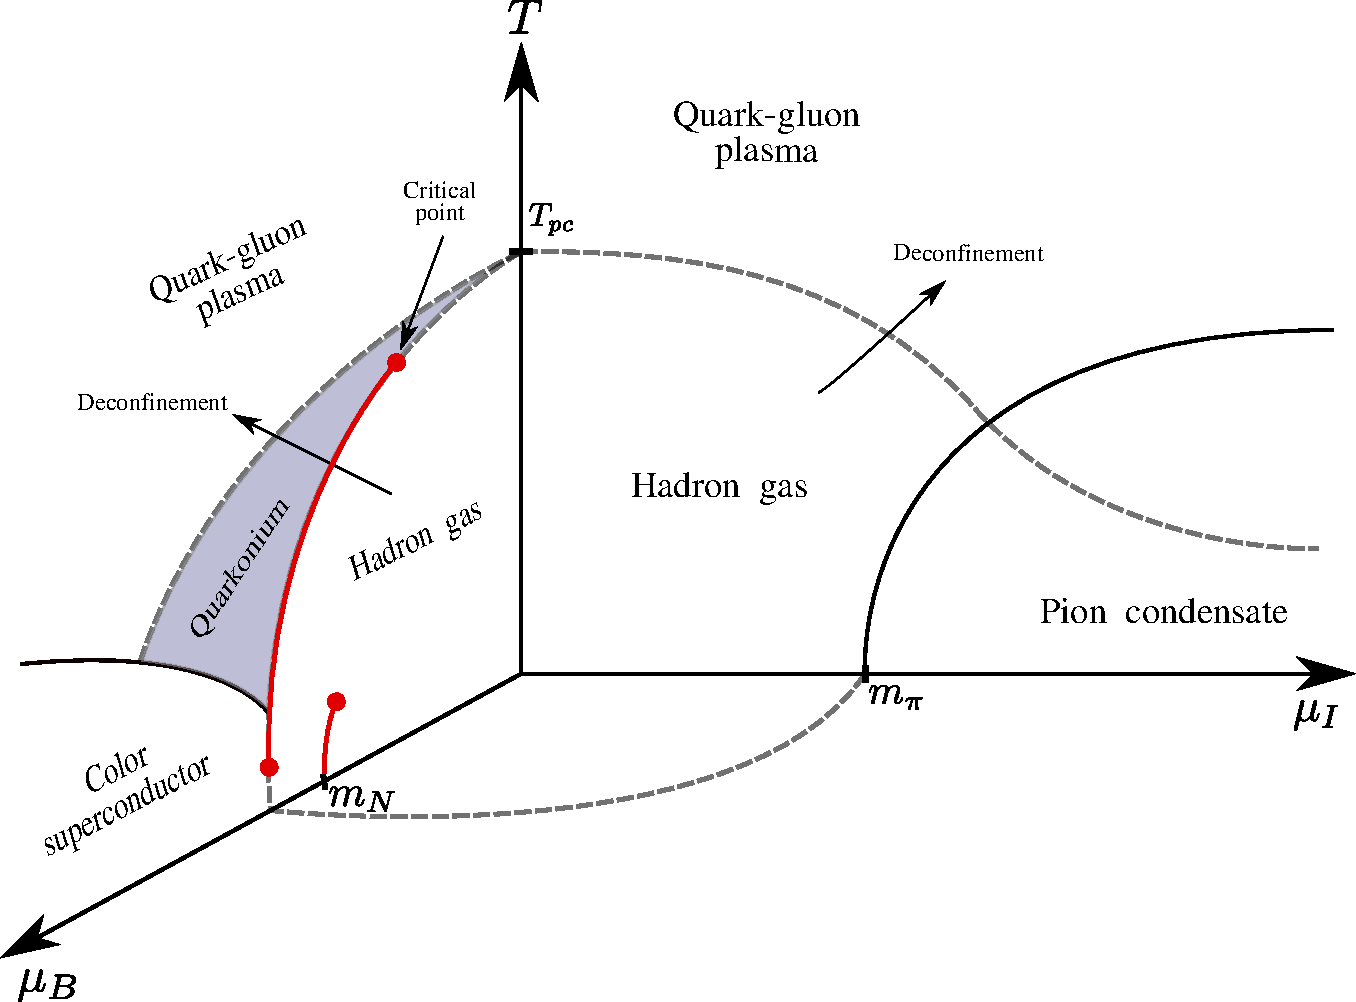
\includegraphics[width=.85\textwidth]{figurer/phase_diagram2.pdf}
    \caption{
        A sketch of the QCD phase diagram based on
        ~\autocite{fukushimaPhaseDiagramDense2010,andronicHadronProductionUltrarelativistic2010,baymHadronsQuarksNeutron2018}.
        See main text for a detailed description.
        }
    \label{fig: phase diagram QCD}
\end{figure}


Close to $T = \mu_B = \mu_I = 0$, QCD is in the vacuum phase, where hadrons form a gas whose density and composition depend on the temperature and chemical potentials.
The first explorations of the phase transitions were done when it was noticed at CERN that hadrons seem to have a maximum temperature, the Hagedorn temperature of around $160\,\text{MeV}$ or $1.9\times 10^{12} \, K$.
A more modern understanding of this temperature is as a point of phase transition, in which the quarks cease to be bound together as hadrons and instead form a soup of nearly free particles called quark-gluon plasma.
This process is called deconfinement and is a consequence of the weakening of the strong force at higher energies, called \emph{asymptotic freedom}
~\autocite{hagedornHadronicMatterBoiling1968,cabibboExponentialHadronicSpectrum1975}.
At zero isospin and baryon chemical potential, this transition called a crossover, is smooth and characterized by a pseudo-critical temperature $T_{pc}$~\autocite{fukushimaPhaseDiagramDense2010}.
Recent lattice QCD results indicate $T_{pc}$ is around $160\, \text{MeV}$~\autocite{borsanyiThereStillAny2010}.
Experimental observation of quark-gluon plasma was first reported by the Relativistic Heavy Ion Collider at Brookhaven National Laboratories in 2006~\autocite{adcoxFormationDensePartonic2005,backPHOBOSPerspectiveDiscoveries2005}.

As the baryon chemical momentum increases, nucleons undergo a gas-liquid transition at low temperatures.
This happens approximately at the nuclear mass, $\mu_I \approx m_N \approx 0.9 \, \text{GeV}$.
As $\mu_B$ is increased further, asymptotic freedom means that perturbative treatments again become available.
Under such conditions, QCD enters a phase analogous to that of an electrical superconductor and forms a \emph{color superconductor}.
Here, quarks at the surface of the Fermi sphere form Cooper pairs, as electrons do in the Bardeen-Cooper-Schrieffer (BCS) theory of electromagnetic superconductors.
Furthermore, there is a color Meissner effect, in which gluons gain mass due to the Higgs mechanism, as the photon does in electromagnetic superconductors.
The transition from the vacuum state to the color superconducting state is not well understood.
Here, the density is still too low for perturbative treatment and numerical lattice calculations are haunted by the \emph{sign problem}.
Lattice methods discretize quantum fields on a finite lattice, representing space-time, then randomly sample configurations using the Metropolis-Hastings algorithm.
This, however, relies on each configuration having a real, positive weight which allows for the inclusion of a minority of important configurations.
For non-zero baryon chemical potential, this is not the case, and lattice methods, therefore, fail~\autocite{troyerComputationalComplexityFundamental2005}.

This problem does not arise in the case of zero baryon chemical potential, but a non-zero isospin chemical potential.
QCD lattice results, therefore, allow for an exploration of the behavior of QCD under non-zero $\mu_I$.
\chpt\, predicts a second order phase transition from the vacuum phase to a pion-condensed phase at $\mu_I = m_\pi$~\autocite{sonQCDFiniteIsospin2001}.
Early lattice calculations agrees with these results~\autocite{kogutQuenchedLatticeQCD2002,kogutLatticeQCDFinite2002,kogutFiniteTemperatureTransition2004,sinclairSearchingElusiveCritical2006}, 
which have been further confiremed by subsequent studies~\autocite{brandtNewClassCompact2018,brandtQCDFiniteIsospin2018,brandtQCDPhaseDiagram2018,brandtReliabilityTaylorExpansions2019,brandtQCDPhaseDiagram2017}.
The pion condensate is characterized by a non-zero condensate with an isospin charge.
This phase is a Bose-Einstein condensed (BEC) phase, in which a zero-momentum state is highly occupied by identical bosons.
At asymptotically large $\mu_I$, it is conjectured that the BEC phase continuously transitions into a deconfined BCS state~\autocite{sonQCDFiniteIsospin2001a,sonQCDFiniteIsospin2001}.




Mapping out the full phase diagram and nature of the critical points and the phase transitions of QCD is one of the most basic questions in physics---what happens to the fundamental building blocks of matter if they are heated up or compressed?
As such, it is an imperative in basic science to extend our knowledge on this subject and to develop a wide array of methods of investigation to check our assumptions.
As stated earlier, the dynamics of stars have always been a great inspiration and guidance for the development of physics.
As the most extreme furnaces in the universe, they serve as an excellent, real-world test for our theoretical understanding of exotic states of matter.
It is believed that the core of neutron stars consists of deconfined quark matter, which could be in a color superconducting phase~\autocite{baymHadronsQuarksNeutron2018,alfordColorSuperconductivityDense2008}.
They may thus play an important part in developing our understanding of the extreme forms of QCD.
The early universe is another place of extreme conditions.
Although the exact conditions are still unclear, it has been shown that the conditions there might have caused pion condensation.
If so, this would leave possibly observable traces in the form of gravitational waves~\autocite{hajkarimEffectsQCDEquation2019,wygasCosmicQCDEpoch2018,vovchenkoPionCondensationEarly2021}.
Furthering our understanding of the pion-condensed phase and the properties of the stars it might form, then, is an important part of a project to map out the behavior of the most fundamental building blocks in the universe and the traces they might have left for us to find.




\section{Outline of theseis}

To make this thesis as self-contained as possible, we have included some parts from the earlier specialization project with only minor modifications.
These parts are therefore marked with an asterisk (*) in the headers and the table of contents.
The parts are \autoref{appendix: two flavor results} and \autoref{appendix: thermal field theory}; from \autoref{section: path integral} to and including \autoref{seciton: ccwz construction} and \autoref{appendix: consisten expansion}; \autoref{section:gaussian integrals}; \autoref{subsection: Weinberg's power counting scheme} and \autoref{subsection: non-linear realization}.
We aim for this to be readable for someone who has the background equivalent of a master's degree in physics and some familiarity with particle physics, quantum field theory, and general relativity, but not necessarily any specific knowledge of chiral perturbation theory or the modeling of compact stars.
This thesis, therefore, contains an extensive introduction to the requisite theory as well as appendices with additional material.

\autoref{part: theoretical background} of this thesis surveys the theoretical foundations of \chpt\, and the modeling of pion stars.
In \autoref{chapter: math}, we summarize the mathematical prerequisites, specifically differential geometry and Lie theory.
We introduce the notion of smooth manifolds and tensor fields.
By introducing the metric, we develop a generalization of calculus to manifolds.
This is then applied to study Lie groups and Lie algebras.
\autoref{chapter: QFT} develops the necessary background in quantum field theory.
We outline the path integral formulation of QFT and apply this to introduce the 1PI effective action, the role of symmetry and the CCWZ construction.
We then discuss the notion of effective field theories, and how to construct one.
In \autoref{chapter: GR} we survey the physics of gravity.
We discuss the Newtonian theory and its successor, general relativity, and apply this to derive the TOV equation of hydrostatic equilibrium.
This is used to study a simple model of neutron stars.

In \autoref{part: chpt and the pion-condensed phase}, we apply the theory to develop and study \chpt.
We start in \autoref{chapter: chpt} by summarizing QCD, which allows us to construct the effective Lagrangian of \chpt\, to leading and next-to-leading order.
We study the spectrum of the resulting particles, and how it is affected by electromagnetic interactions and a non-zero isospin and strangeness chemical potential.
In \autoref{chapter: thermodynamics}, we investigate the thermodynamic properties of the condensed phases of \chpt.
We draw the phase diagram in the $\mu_I-\mu_S$ plane and discuss the effect of EM interactions.
The nature of the phase transitions is discussed.
Furthermore, we calculate the equation of state of the pion-condensed phase to leading and next-to-leading order, and in a charge-neutral system including charged leptons and neutrons.

Finally, our results are applied to model pion stars in \autoref{part: pion stars}.
In \autoref{chapter: pion stars}, we use the equations of state we found together with the TOV equation to calculate the pressure and energy profile of pion stars, as well as the mass-radius relation.
We discuss how the different compositions and orders in perturbation theory affect the resulting stars and compare our results to earlier numerical calculations.
In \autoref{Chapter: cocnlusion and discussion}, we summarize our results and discuss ways to improve them and avenues for further research.

The appendices include definitions, derivations, and background theory left out of the main text.
\autoref{appendix: A} include the numerical values of physical constants, the properties and explicit forms of algebras used in the text as well as additional derivations.
\autoref{appendix: two flavor results} and \autoref{appendix: thermal field theory} are parts of the specialization project included as supplemental material.
\autoref{appendix: two flavor results} details theory and results for the two-flavor case of \chpt, while \autoref{appendix: thermal field theory} summarizes thermal field theory.
The code used to derive the results of this thesis is discussed in \autoref{appendix: code}, where we also link to an online repository where it is available in full.
The appendices are referenced in the main text when relevant.

